%%%%%%%%%%%%%%%%%%%%%%%%%%%%%%%%%%%%%%%%%%%%%%%%%%%%%%%%%%%%%%%%%%%%
%%%%%%%%%%%%%%%%%%%%%%%%%%%%%%%%%%%%%%%%%%%%%%%%%%%%%%%%%%%%%%%%%%%%
%%                                                                %%
%% Esimerkki opinnäytteen tekemisestä LaTeX:lla 20130926          %%
%% Alkuperäinen versio Luis Costa,  muutokset Perttu Puska        %%
%%                                                                %%
%% Tähän esimerkkiin kuuluu tiedostot                             %%
%%               opinnaytepohja.tex (versio 1.7)                  %%
%%               aaltothesis.sty (versio 1.7)                     %%
%%               kuva1.eps                                        %%
%%               kuva2.eps                                        %%
%%                                                                %%
%%                                                                %%
%% Kääntäminen                                                    %%
%% latex:                                                         %%
%%             $ latex opinnaytepohja                             %%
%%             $ latex opinnaytepohja                             %%
%%                                                                %%
%%   Tuloksena on tiedosto opinnayte.dvi, joka                    %%
%%   muutetaan ps-muotoon seuraavasti                             %%
%%                                                                %%
%%             $ dvips opinnaytepohja -o                          %%
%%                                                                %%
%% Selittävät kommentit on tässä esimerkissä varustettu           %%
%% %%-merkeillä ja muutokset, joita käyttäjä voi tehdä,           %%
%% on varustettu %-merkeillä                                      %%
%%                                                                %%
%%%%%%%%%%%%%%%%%%%%%%%%%%%%%%%%%%%%%%%%%%%%%%%%%%%%%%%%%%%%%%%%%%%%
%%%%%%%%%%%%%%%%%%%%%%%%%%%%%%%%%%%%%%%%%%%%%%%%%%%%%%%%%%%%%%%%%%%%

%% Käytä toinen näistä, jos kirjoitat suomeksi:
%% ensimmäinen, jos käytät pdflatexia (kuvat on oltava pdf-tiedostoina)
%% toinen, jos haluat tuottaa ps-tiedostoa (käytä eps-formaattia kuville).
%%
%% Use one of these you write in Finnish:
%% the 1st when using pdflatex (use pdf figures) or
%% the 2nd when producing a ps file (use eps figures).
\documentclass[finnish,12pt,a4paper,pdftex]{article}
%\documentclass[finnish,12pt,a4paper,dvips]{article}

%% Käytä näitä, jos kirjoitat englanniksi
%%
%% Uncomment one of these if you write in English
%\documentclass[english,12pt,a4paper,pdftex]{article}
%\documentclass[english,12pt,a4paper,dvips]{article}

%% Tämä paketti on pakollinen
%% Valitse korkeakoulusi näistä: arts, biz, chem, elec, eng, sci.
%% Valiste editorisi käyttämä merkkikoodaustapa: utf8, latin1
%%
%% This package is required
%% Choose your school from arts, biz, chem, elec, eng, sci.
%% Choose the character encoding scheme used by your editor: utf8, latin1
\usepackage[elec,utf8]{aaltothesis} % this is the default in aaltothesis.sty
%\usepackage[elec,latin1]{aaltothesis}

%% Jos käytät latex-komentoa käännettäessä (oletusarvo), 
%% kuvat kannattaa tehdä eps-muotoon. Älä käytä ps-muotoisia kuvia!
%% Käytä seuraavaa latex-komennon ja eps-kuvien kanssa 
%%
%% Jos taas käytät pdflatex-komentoa, joka kääntää tekstin suoraan
%% pdf-tiedostoksi, kuvasi on oltava jpg-formaatissa tai pdf-formaatissa.
%%
%% Use this if you run pdflatex and use jpg/pdf-format pictures.
%%
\usepackage{graphicx}
\usepackage{datetime}
%% Jos et jostain syystä pidä, miten alla oleva hyperref-paketti käyttää
%% fontteja, värejä yms., käytä tämän paketin makroja muuttamaan
%% fonttimäärittelyt. Katso paketin dokumentaatiota. Paketti määrittelee
%% \url-makron, joten ota paketti käyttöön, jos et käytä hyperref-pakettia.
%%
%% Use the macros in this package to change how the hyperref package below 
%% typesets its hypertext -- hyperlink colour, font, etc. See the package
%% documentation. It also defines the \url macro, so use the package when 
%% not using the hyperref package.
%\usepackage{url}

%% Saat pdf-tiedoston viittaukset ja linkit kuntoon seuraavalla paketilla.
%% Paketti toimii erityisen hyvin pdflatexin kanssa. 
%%
%% Use this if you want to get links and nice output with pdflatex
\usepackage[pdfpagemode=None,colorlinks=true,urlcolor=red,%
linkcolor=blue,citecolor=black,pdfstartview=FitH]{hyperref}

%% Matematiikan fontteja, symboleja ja muotoiluja lisää, näitä tarvitaan usein 
%%
%% Use this if you write hard core mathematics, these are usually needed
\usepackage{amsfonts,amssymb,amsbsy}  
\usepackage{graphicx}

\hyphenpenalty=100000
\setlength{\parindent}{0em}
\setlength{\parskip}{1em}

%% Vaakasuunnan mitat, ÄLÄ KOSKE!
\setlength{\hoffset}{-1in}
\setlength{\oddsidemargin}{35mm}
\setlength{\evensidemargin}{25mm}
\setlength{\textwidth}{15cm}
%% Pystysuunnan mitat, ÄLÄ KOSKE!
\setlength{\voffset}{-1in}
\setlength{\headsep}{7mm}
\setlength{\headheight}{1em}
\setlength{\topmargin}{25mm-\headheight-\headsep}
\setlength{\textheight}{23cm}
\usepackage[
    %backend=biber, 
    natbib=true,
    style=numeric-comp,
    sorting=none
]{biblatex}
\bibliography{sources}


%% Kaikki mikä paperille tulostuu, on tämän jälkeen
%%
%% Output starts here
\begin{document}

%% Korjaa vastaamaan korkeakouluasi, jos automaattisesti asetettu nimi on 
%% virheellinen 
%%
%% Change the school field to describe your school if the autimatically 
%% set name is wrong
% \university{aalto University}{aalto-Yliopisto}
% \school{School of Electrical Engineering}{SähköTekniikan korkeakoulu}

%% Vain kandityölle: Korjaa seuraavat vastaamaan koulutusohjelmaasi
%%
%% Only for B.Sc. thesis: Choose your degree programme. 
\degreeprogram{Electronics and electrical engineering}%
{Elektroniikka ja sähkötekniikka}
%%

%% Vain DI/M.Sc.- ja lisensiaatintyölle: valitse laitos, 
%% professuuri ja sen professuurikoodi. 
%%
%% Only for M.Sc. and Licentiate thesis: Choose your department,
%% professorship and professorship code. 
%\department{Department of Radio Science and Technology}%
%{Radiotieteen ja -tekniikan laitos}
%\professorship{Circuit theory}{Piiriteoria}
%\code{S-55}
%%

%% Valitse yksi näistä kolmesta
%%
%% Choose one of these:
\univdegree{BSc}
%\univdegree{MSc}
%\univdegree{Lic}

%% Oma nimi
%%
%% Should be self explanatory...
\author{Aarni Halinen}

%% Opinnäytteen otsikko tulee vain tähän. Älä tavuta otsikkoa ja
%% vältä liian pitkää otsikkotekstiä. Jos latex ryhmittelee otsikon
%% huonosti, voit joutua pakottamaan rivinvaihdon \\ kontrollimerkillä.
%% Muista että otsikkoja ei tavuteta! 
%% Jos otsikossa on ja-sana, se ei jää rivin viimeiseksi sanaksi 
%% vaan aloittaa uuden rivin.
%% 
%% Your thesis title. If the title is very long and the latex 
%% does unsatisfactory job of breaking the lines, you will have to
%% break the lines yourself with \\ control character. 
%% Do not hyphenate titles.
\thesistitle{Iot cabable data transfer in LTE/3G-systems}{IoT-soveltuva tiedonlähetys LTE/3G-järjestelmissä}

\place{Espoo}
%% Kandidaatintyön päivämäärä on sen esityspäivämäärä! 
%% 
%% For B.Sc. thesis use the date when you present your thesis. 

\newdateformat{specialdate}{\twodigit{\THEDAY}.\twodigit{\THEMONTH}.\THEYEAR}
\date{\specialdate\today}
%\date{\today}

%% Kandidaattiseminaarin vastuuopettaja tai diplomityön valvoja.
%% Huomaa tittelissä "\" -merkki pisteen jälkeen, 
%% ennen välilyöntiä ja seuraavaa merkkijonoa. 
%% Näin tehdään, koska kyseessä ei ole lauseen loppu, jonka jälkeen tulee 
%% hieman pidempi väli vaan halutaan tavallinen väli.
%%
%% B.Sc. or M.Sc. thesis supervisor 
%% Note the "\" after the comma. This forces the following space to be 
%% a normal interword space, not the space that starts a new sentence. 
\supervisor{Lecturer\ Markus Turunen}{Leht.\ Markus Turunen}

%% Kandidaatintyön ohjaaja(t) tai diplomityön ohjaaja(t)
%% 
%% B.Sc. or M.Sc. thesis advisors(s). 
%%
%% Note that there has been a change in the official EN translation
%% of the Finnish title ``ohjaaja'' which in the previous version (1.5) 
%% of this document was called ``instructor''. The recommended
%% translation is now ``advisor''.  
%% However, the LaTeX internal variable remains \instructor
%% as there is little point to change the variable name. 
%%
\instructor{Lecturer\ Kalle Ruttik}{Leht.\ Kalle Ruttik}

%% Aaltologo: syntaksi:
%% \uselogo{aaltoRed|aaltoBlue|aaltoYellow|aaltoGray|aaltoGrayScale}{?|!|''}
%% Logon kieli on sama kuin dokumentin kieli
%%
%% Aalto logo: syntax:
% \uselogo{aaltoRed|aaltoBlue|aaltoYellow|aaltoGray|aaltoGrayScale}{?|!|''}
%% Logo language is set to be the same as the document language.
\uselogo{aaltoRed}{''}

%% Tehdään kansilehti
%%
%% Create the coverpage
\makecoverpage{}

%
%% English abstract, uncomment if you need one. 
%% 
%% Abstract keywords
%\keywords{NB-IoT}
%% Abstract text
%\begin{abstractpage}[english]
%% Your abstract in English. Try to keep the abstract short, approximately 
%% 100 words should be enough. Abstract explains your research topic, 
%% the methods you have used, and the results you obtained.  

%\end{abstractpage}
%% Note that 
%% if you are writting your master's thesis in English place the English
%% abstract first followed by the possible Finnish abstract



%% Pakotetaan uusi sivu varmuuden vuoksi, jotta 
%% mahdollinen suomenkielinen ja englanninkielinen tiivistelmä
%% eivät tule vahingossakaan samalle sivulle
%%
%% Force new page so that English abstract starts from a new page
\newpage

%% Suomenkielinen tiivistelmä
%% 
%% Finnish abstract
%%
%% Tiivistelmän avainsanat
\keywords{IoT, LTE, M2M, NB-IoT}
%% Tiivistelmän tekstiosa
\begin{abstractpage}[finnish]

\end{abstractpage}

%% Esipuhe 
%%
%% Preface
%%\mysection{Esipuhe}
%\mysection{Preface}
%%Haluan kiittää Professori Pirjo Professoria ja ohjaajaani Olli Ohjaajaa hyvästä ja huonosta ohjauksesta.\\

%\vspace{5cm}
%Otaniemi, 24.9.2013

%\vspace{5mm}
%{\hfill Teemu T.\ A.\ Teekkari \hspace{1cm}}

%% Pakotetaan varmuuden vuoksi esipuheen jälkeinen osa
%% alkamaan uudelta sivulta
%%
%% Force new page after preface
\newpage


%% Sisällysluettelo
%% 
%% Table of contents. 
\thesistableofcontents{}


%% Symbolit ja lyhenteet
%%
%% Symbols and abbreviations
\mysection{Symbolit ja lyhenteet}

%\mysection{Symbols and abbreviations}
%\subsection*{Symbolit}
%\subsection*{Symbols}

%\begin{tabular}{ll}
%$|a_{ij}|^2$, $|a_i|^2$ & probability of two electrons having momenta
%    $\boldsymbol p_i$ and $\boldsymbol p_j$ ($\boldsymbol p_i$ for $|a_i|^2$) \\
%                 & at any given instant \\
%%$\mathbf{B}$  & magneettivuon tiheys  \\
%%$c$              & valon nopeus tyhjössä $\approx 3\times10^8$ [m/s]\\
%$p$              & magnitude of momentum \\
%$\boldsymbol p$, $\boldsymbol p_i$, $\boldsymbol p_i^{'}$  & momentum vector \\
%$p$              & magnitude of momentum \\
%$\boldsymbol p$, $\boldsymbol p_i$, $\boldsymbol p_i^{'}$  & momentum vector \\
%$\boldsymbol P$  &  \\
%$p_{\mathrm{F}}$ & Fermi momentum \\
%%$\omega_{\mathrm{D}}$    & Debye-taajuus \\
%%$\omega_{\mathrm{latt}}$ & hilan keskimääräinen fononitaajuus \\
%%$\uparrow$       & elektronin spinin suunta ylöspäin\\
%%$\downarrow$     & elektronin spinin suunta alaspäin
%\end{tabular}

%\subsection*{Operaattorit}
%\subsection*{Opetators}

%\begin{tabular}{ll}
%%$\nabla \times \mathbf{A}$              & vektorin $\mathbf{A}$ roottori\\
%%$\displaystyle\frac{\mbox{d}}{\mbox{d} t}$ & derivaatta muuttujan $t$ suhteen\\
%%[3mm]
%%$\displaystyle\frac{\partial}{\partial t}$  & osittaisderivaatta muuttujan $t$ suhteen \\[3mm]
%%$\sum_i $                       & Summa indeksin $i$ yli\\
%%$\mathbf{A} \cdot \mathbf{B}$    & vektorien $\mathbf{A}$ ja $\mathbf{B}$ pistetulo
%\end{tabular}

\subsection*{Lyhenteet}
%\subsection*{Abbreviations}

\begin{tabular}{ll}
3G & 3rd Generation \\
3GPP & 3rd Generation Partnership Project \\
4G & 4th Generation \\
CDMA & Code Division Multiple Access \\
CFI & Control Format Indicator \\
CRC & Cylic Redundancy Check \\
CRS & Cell-specific Reference Signal \\
D2D & Device-to-Device \\
EDGE & Enhanced Data rates for GSM Evolution \\
FDD & Frequency-Division Duplex \\
FDMA & Frequency-Division Multiple Access \\
GERAN & GSM EDGE Radio Access Network \\
GSM & Global System for Mobile Communications \\
H2H & Human-To-Human \\
IoT & Internet of Things \\
LPWA & Low-Power Wide-Area \\
LTE & Long-Term Evolution \\
LTE-A & Long-Term Evolution Advanced \\
LTE-M & LTE for M2M \\
M2M & Machine-to-Machine \\
MAC & Medium Access Control \\
MIB & Master Information Block \\
NB-IOT & NarrowBand Internet of Things \\
NB LTE-M & NarrowBand LTE-M for M2M \\
NPBCH & NarrowBand Physical Broadcast Channel \\
NPDCCH & NarrowBand Physical Downlink Control Channel \\
NPDSCH & NarrowBand Physical Downlink Shared Channel \\
NPRACH & NarrowBand Physical Random Access Channel \\
NPUCCH & NarrowBand Physical Uplink Control Channel \\
NPUSCH & NarrowBand Physical Uplink Shared Channel \\
NPSS & NarrowBand Primary Synchronization Signal \\
NSSS & NarrowBand Secondary Synchronization Signal \\
OFDM & Orthogonal Frequency-Division Multiplexing \\
PCFICH & Physical Control Format Indicator Channel \\
PCID & Physical Cell ID \\
PDCCH & Physical Downlink Control Channel \\
PHICH & Physical Hybrid ARQ Indicator Channelvii \\
PMCH & Physical Multicast Channel \\
PRACH & Physical Random Access Channel \\
PRB & Physical Resource Block \\
RAN & Random Access Network \\
RRC & Radio Resource Control \\
SIB & System Information Block \\
UMTS & Universal Mobile Terrestrial System \\
TBCC & Tail-Biting Convolutional Code \\
TDD & Time-Division Duplex \\
UTRA & Universal Terrestrial Radio Access \\
QAM & Quadrature Amplitude Modulation \\
QPSK & Quadrature Phase Shift Keying \\
\end{tabular}


%% Sivulaskurin viilausta opinnäytteen vaatimusten mukaan:
%% Aloitetaan sivunumerointi arabialaisilla numeroilla (ja jätetään
%% leipätekstin ensimmäinen sivu tyhjäksi, 
%% ks. alla \thispagestyle{empty}).
%% Pakotetaan lisäksi ensimmäinen varsinainen tekstisivu alkamaan 
%% uudelta sivulta clearpage-komennolla. 
%% clearpage on melkein samanlainen kuin newpage, mutta 
%% flushaa myös LaTeX:n floatit 
%% 
%% Corrects the page numbering, there is no need to change these
\cleardoublepage{}
\storeinipagenumber{}
\pagenumbering{arabic}
\setcounter{page}{1}

%% Ensimmäinen sivu tyhjäksi
%% 
%% Leave first page empty
%%\thispagestyle{empty}
%%\newpage

%% Leipäteksti alkaa
%%
%% Text body begins. Note that since the text body
%% is mostly in Finnish the majority of comments are
%% also in Finnish after this point. There is no point in explaining
%% Finnish-language specific thesis conventions in English.
\section{Johdanto}
%\section{Introduction}

Esineiden internetillä (Internet of things, IoT) tarkoitetaan laitteiden välistä yhteyttä ja tiedonsiirtoa internetin avulla. Se mahdollistaa uudenlaisia palveluita mm. turvallisuuden, laitteiden huollon ja päivittämisen sekä älykkäiden verkkojen saralla. Esineiden internetin myötä verkkoon kytkettyjen laitteiden määrä kasvaa räjähdysmäisesti 2020-luvulle mentäessä. Arviolta 50 miljardia laitetta on kytketty internetiin vuonna 2020 \cite{ratasuk2016nb}.

Verkon liikenteestä suuren osan tulee muodostamaan erilaiset sensorit, jotka viestivät palvelimien ja muiden IoT-laitteiden kanssa. Tehokas laitteiden välinen kommunikaatio (M2M) on välttämätön edellytys toimivalle IoT-infrastruktuurille. IoT-laitteiden tiedonsiirto koostuu pääosin pienistä datalähetyksistä, joita lähetetään varsin harvoin. Laitteiden toiminnalle on tärkeää, että laitteen ja verkon välinen kommunikaatio ei kuluta resursseja turhaan. Kommunikaatio ei myöskään saa rasita verkkoa liikaa. \cite{nokiawhitepaper}

3rd Generation Partnership Projectin standardoimaan Long Term Evolution --järjestelmään (LTE) on muutaman viime vuoden aikana tehty useita päivityksiä tukemaan IoT-laitteille sopivaa, pienen tehonkulutuksen kommunikaatiota. LTE:n \textit{Release 12} \cite{release12} esitteli LTE-M teknologian keskisuuria tiedonsiirtonopeuksia ja liikkuvia IoT-laitteita varten \cite{ratasuk2016overview}. \textit{Release 13}:ssa \cite{release13} esiteltiin Narrowband IoT (NB-IoT) matalan kompleksisuuden laitteille, sekä paranneltiin LTE-M-teknologiaa. NB-IoT:n on tarkoitus tarjota halpoja laitteistototeutuksia, yli 10 vuoden akunkestoa IoT-laitteille, sekä mahdollisuus kytkeä yli 52 tuhatta laitetta samanaikaisesti samalle kanavalle \cite{nokiawhitepaper}. Koska NB-IoT on kehitelty jo olemassa olevia LTE-toteutksia hyödyntäväksi, on se myös mahdollista ottaa käyttöön vähäisin kustannuksin.

Tämän työn tarkoitus on tutkia, miten LTE-järjestelmiä on muokattu tukemaan IoT-datalähetyksiä. Tutkimus toteutetaan kirjallisuustutkimuksena. Toisessa luvussa käsitellään M2M-kommunikaatiota ja kartoitetaan IoT-laitteiden asettamia vaatimuksia verkoille. Kolmannessa luvussa käsitellään LTE-järjestelmän standardointia ja esineiden internetille tärkeimpiä viimeaikaisia muutoksia niihin. Neljännessä luvussa tutustutaan tuoreimpiin LTE-julkaisuihin IoT-laitteiden näkökulmasta ja tämän pohjalta pohditaan, mihin suuntaan kehitystyö jatkuu.

%% Opinnäytteessä jokainen osa alkaa uudelta sivulta, joten \clearpage
%%
%% In a thesis, every section starts a new page, hence \clearpage
\clearpage
\section{M2M-kommunikaatio}
%\section{M2M communication}

\subsection{Esineiden internet (IoT)}

Esineiden internet -termi kehitettiin vuonna 1999 kuvaamaan RFID-tunnisteilla varustettujen laitteiden globaalia verkkoa \cite{sundmaeker2010vision}. Termi on nykyään laajentunut määrittelemään esineiden muodostama verkkoa, jossa laitteet keräävät ja lähettävät tietoa toisilleen. \cite{atzori2010internet}. Verkon esineet voivat olla kaikkea suurista teollisuuden laitteista sensoreihin tai puettaviin tietokoneisiin, kuten älykelloihin. Autonomisesti toisilleen viestivät laitteet mahdollistavat laitteille parempaa tehokkuutta sekä parannuksia käyttäjäkokemukseeen. Tämä laitteiden välinen kommunikaatio, eli niin sanottu Machine-to-machine -kommunikaatio (M2M), on edellytys esineiden internetin muodostamiselle \cite{nokiawhitepaper}.

%\begin {figure}[h!]
%    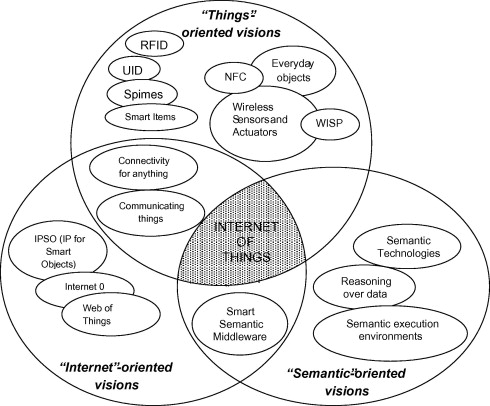
\includegraphics[width=\linewidth]{IoT.jpg}
%    \caption{Esineiden internet eri näkökulmista. \cite{atzori2010internet}}
%    \label{fig:IoT}
%\end {figure}

%Esineiden internet voidaan jakaa 

Esineiden internetin päätelaitteiden tuottama verkkoliikenne voidaan jakaa kiinteän ja lyhyen kantaman liikenteeseen, mobiiliverkkojen ja LPWA-verkkojen (Low-Power Wide-Area) kautta kulkevaan liikenteeseen \cite{nokiawhitepaper, harmaala}. Päätelaitteista suurin osa kommunikoi kiinteän ja lyhyen kantaman yhteyksiä hyväksi käyttäen \cite{nokiawhitepaper}. Tällaisia yhteyksiä ovat muun muassa Bluetooth ja Near-field-communication (NFC). Kuitenkin noin 7 miljardia laitetta kommunikoi käyttäen perinteisiä mobiili- sekä LPWA-verkkoja \cite{nokiawhitepaper}.

LPWA-verkot on jaettu 3GPP:n standardoinnin ulkopuolisiin, lisenssoimattomiin verkkoihin, kuten SigFox ja LoRa, sekä 3GPP:n lisenssoimiin cellular-IoT teknologioihin \cite{nokiawhitepaper}. 3GPP:n lisenoimia teknologioita ovat \textit{Release 12}:ssa julkaistu LTE-M sekä \textit{Release 13}:n esittelemä NB-IoT. Tässä luvussa esitellään mobiiliverkkoa hyödyntävien IoT-laitteiden asettamia haasteita ja edellytyksiä LTE-verkolle.

\subsection{M2M-kommunikaation edellytykset LPWA-verkoille}

LPWA-verkot ovat tärkeässä roolissa turvallisten, pienitehoisten, pitkän kantaman ja alhaisen hinnan laitteiden yhdistämisessä osaksi esineiden internetiä \cite{gsmawhitepaper}. Tällaisia palveluja ovat muun muassa logistiikkaan, älykkäisiin kaupunkeihin, maanviljelyyn ja ympäristöön ja infrastruktuuriin liittyvät palvelut. Näitä palveluita yhdistää useimmiten tarve laajalle verkon kattavuudelle, kuuluvuudelle myös sisätiloissa ja yhteyden puuttuminen verkkovirtaan \cite{gsmawhitepaper}. Jotta palveluiden M2M-kommunikaatio olisi mahdollista ja taloudellisesti järkevää, LPWA-verkon tulee mahdollistaa päätelaitteille pitkä akunkesto ja laaja maantieteellinen peitto, samalla tukien suurta laitemäärää ja pitäen päätelaitteiden laitteisto- ja kehityskustannukset matalina.

Akunkeston pidentämistä voidaan pitää merkittävimpänä haasteena verkolle, sillä päätelaite voi olla vaikeakulkuisessa paikassa tai jatkuvassa liikkeessä. Akun vaihtaminen on täten työlästä ja kallista, minkä lisäksi pitkä akunkesto mahdollistaa uusien palvelujen kehittämisen \cite{nokiawhitepaper}. Päivittäin dataa keräävän ja pieninä paketteina lähettävän laitteen akun tavoitekestona pidetään alalla yleisesti vähintään 10 vuotta. 

Verkon kattavuus on tärkeää monille IoT-laitteille, jotka saattavat sijaita rakennusten kellareissa tai muilla verkon katvealueilla \cite{nokiawhitepaper}. Esimerkiksi hissit ja liukuhihnat voivat toimia sisätiloissa paksujen seinien peittäminä. Heikommpaa signaalin voimakkuutta sietävät päätelaitteet, suunnatut antennit sekä päätelaitteiden kommunikaation ketjutus (LTE D2D) ovat ratkaisuja kattavuuden parantamiseksi \cite{nokiawhitepaper, diaz20163gpp}.% 15--20 dB:n parannus signaalille vastaisi seinien läpäisystä aiheutuvaa vaimennusta \cite{nokiawhitepaper}.

Esineriden internetin myötä verkkoon kytekttyjen laitteiden määrä kasvaa, ja vuoteen 2025 mennessä LPWA-verkkoihin on kytkettynä noin 7 miljardia IoT-laitetta, mikä vastaa nykyhetken globaalin mobiililittymien tilaajamäärää \cite{nokiawhitepaper}. Lisääntynyt liikenne voi ruuhkauttaa verkoa, mikä vaikuttaa koneiden välisen liikenteen lisäksi myös ihmisten väliseen liikenteeseen hidastaen sitä \cite{diaz20163gpp}. Kaikki verkon laitteet eivät myöskään jakaudu tasaisesti solujen välille, joten yksittäisen verkon solun täytyy pystyä tukemaan hyvin suurta laitemäärää \cite{nokiawhitepaper}. Jo yhden solun ylikuormitus heikentää myös muiden solujen suorituskykyä.

Alhaiset päätelaitekustannukset ovat tärkeä osa LPWA-verkon houkuttelevuutta. IoT-palveluntarjoajille on tärkeää, että LPWA-verkkoon kyetään yhdistämään matalan kompleksisuuden laitteilla, sillä palveluntarjoajien liiketoiminta perustuu usein lukuisien sensorien keräämään dataan. Tavoitteena alalla on alle viiden dollarin hinta moduulille \cite{nokiawhitepaper}. Laitekustannusten lisäksi verkkoon yhdistämisen tulee olla mahdollisimman edullista, jotta palveluiden pariin on mahdollista houkutella riittävästi alhaisista hintaluokasta kiinnostuneita asiakkaita \cite{harmaala}. Lisäksi LPWA-verkon pystyttämisen hinta tulee pitää hinnaltaan alhaisena. LTE-järjestelmissä LPWA-verkko kyetään toteuttamaan olemassa olevalle laitteistolle ohjelmistopäivityksenä, joten verkolle ei tarvita laitteistohankintoja \cite{nokiawhitepaper}.

%Security

\clearpage
\section{LTE-järjestelmän standardointi}

\subsection{Standardointiprosessi}

LTE-standardin kehityksestä ovat yhteistyössä vastuussa 3rd Generation Partnership Project (3GPP), European Telecommunications Standards Institute (ETSI), Oen Mobile Alliance (OMA), China Communications Standards Association (CCSA) ja Alliance for Telecommunications Industry Solution (ATIS). Edellä mainituista instituutioista 3GPP on vastuussa M2M-kommunikaation sulauttamisesta osaksi mobiiliverkkoja, kun taas vastaavasti ETSI:n vastuulla on M2M-kommunikaation palveluarkkitehtuuri. \cite{ghavimi2015m2m}

3GPP:n tavoitteena kehitystyössä on muokata LTE-järjestelmän ydinverkkoa (SAE) tukemaan paremmin M2M-kommunikaatiota. Ensimmäiset M2M-kommunikaation mahdollistavat järjestelmäparannukset julkaistiin \textit{Release 10}:ssä, kun verkon rungoksi valittiin Universal Mobile Terrestrial System (UMTS) ja LTE-Advanced -verkot (LTE-A). \textit{Release 10} standardin tavoitteena M2M-kommunikaation osalta oli optimoida järjestelmän kykyä käsitellä M2M-signaloinnin ruuhkan ja verkon ylikuormittumisesta aiheutivia ongelmia. \textit{Release 10}:n jälkeen 3GPP:n kehitysprosessin pääpaino on siirtynyt standardoidun järjestelmäverkon arkkitehtuuriparannuksien tutkimiseen. Tutkimuksen tavoitteena on tunnistaa tarvittavat verkon kehityskohteet ja M2M-palveluiden kannalta olennaisimmat tekijät, jotta verkkoinfastruktuuri pystyisi tukemaan mahdollisimman suurta yhtäaikaista päätelaitteiden määrää. \cite{ghavimi2015m2m}

%\subsection{Standardoinnin tavoitteet}

%\cite{nokiawhitepaper, sharawi2010rf}

\subsection{LTE-järjestelmän kehysrakenne}

\textit{Release 8}:ssa on LTE-järjestelmille määritelty kaksi kehysrakennetta, joiden avulla LTE-järjestelmät ja liikenne tukiasemien ja päätelaitteiden välillä pysyy synkronoituna. Tyypin yksi (kuva \ref{fig:type1}) kehysrakenne tukee taajuusjakoista kaksisuuntaisuutta (FDD), kun taas tyypin kaksi (kuva \ref{fig:type2}) kehysrakenne on aikajakoista kaksisuuntaisuutta (TDD) varten. Molempien kehysrakenteiden lataus- ja lähetyslinkkien aikaintervallit ilmaistaan perusaikayksikön \begin{equation}
    T_s = \frac{1}{1500 \cdot 2048}
\end{equation}
monikertoina. Täten yksi radiokehys on kestoltaan
\begin{equation}
    T_f = 307200 \cdot T_s = 10 ms.
\end{equation}\cite{ETSIts36211}

Tyypin 1 radiokehys on soveltuva niin vuoro- että kaksisuuntaiseen liikenteeseen (half-duplex, full duplex). Jokainen radiokehys on jaettu 20:een, \begin{equation}
    T_{slot} = \frac{T_f}{20} = 0,5 ms
\end{equation}
pituisiin osiin, jotka on numeroitu välillä 0--19. Alikehyksellä tarkoitetaan kahta peräkkäistä radiokehyksen osaa. Jokaisella 10 millisekunnin radiokehyksellä on 10 alikehystä varattu lähetyslinkille ja toiset 10 latauslinkille. Linkit on erotettu toisistaan taajuustasossa, minkä vuoksi vuorosuuntaisessa liikenteessä päätelaitteet eivät pysty lähettämään ja vastaanottamaan samanaikaisesti. \cite{ETSIts36211}
~\begin{figure}[h!]
    \centering
    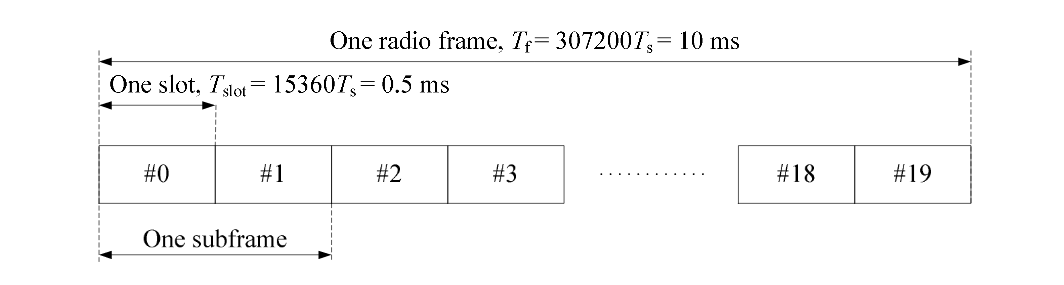
\includegraphics[width=\linewidth]{Images/radioframe1.png}
    \caption{Tyypin yksi LTE-radiokehyksen rakenne. \cite{ETSIts36211}}
    \label{fig:type1}
\end{figure}

Tyypin 2 radiokehys on käytössä aikajakoiselle liikenteelle. Sen 10 millisekunnin kehys on jaettu kahteen 5 millisekunnin puolikehykseen, jotka on puolestaan jaettu viiteen, yhden millisekunnin pituisiin, alikehykseen. \cite{ETSIts36211}
~\begin{figure}[h!]
    \centering
    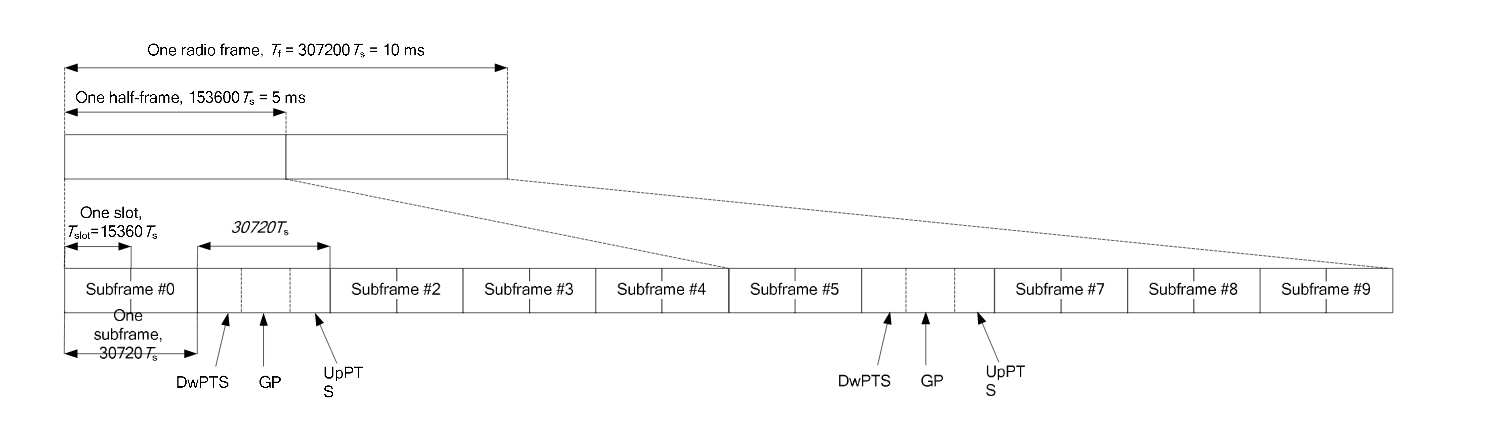
\includegraphics[width=\linewidth]{Images/radioframe2.png}
    \caption{Tyypin kaksi LTE-radiokehyksen rakenne. \cite{ETSIts36211}}
    \label{fig:type2}
\end{figure}

LTE-järjestelmän lähettämät signaalit voidaan kuvailla kuvan \ref{fig:PRB} mukaisella resurssilohkolla. Lohkon pienimpiä aika-taajuus --ykiskköjä kutsutaan resurssielementeiksi, ja niistä jokainen on tunnistettavissa indeksiparin $(k,l)$
\begin{equation}
    k = 0, ..., N^{DL}_{RB}N^{RB}_{SC} -1
\end{equation} 
ja
\begin{equation}
    l = 0, ..., N^{DL}_{symb} -1
\end{equation}
avulla. Resurssielementti jossain tietyssä antenniportissa $p$ voidaan ilmaista kompleksiluvulla $a_{k,l}^{(p)}$. Elementit, joita ei käytetä fyysisen kanavan tai signaalin lähettämiseen tulee olla asetettuna nollaksi. \cite{ETSIts36211}
~\begin{figure}[h!]
    \centering
    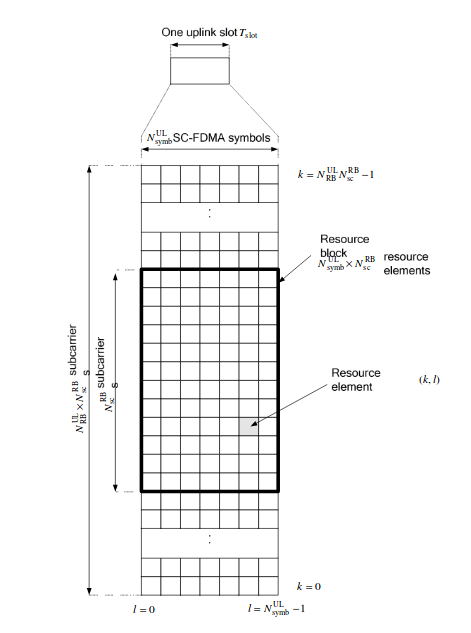
\includegraphics[scale=0.5]{Images/ResourceBlock.png}
    \caption{LTE-järjestelmän resurssilohko (Resource block) radiokehyksessä.\cite{ETSIts36211}}
    \label{fig:PRB}
\end{figure}

\subsection{LTE ja M2M}

M2M-sovellukset eroavat merkittävästi H2H-tyyppisestä (Human-to-Human) kommunikaatiosta, minkä takia alunperin H2H-kommunikaation tarkoitettua LTE-järjestelmää on jouduttu muokkaamaan M2M-sovelluksia varten. Tyypilliset M2M-sovellukset koostuvat älykkäistä sensoreista, joiden liikenne koostuu pääosin pienistä määristä dataa. LTE- ja LTE-A-standardit suunniteltiin alunperin vain laajakaistaisten sovellusten käyttöön, eikä niiden hyödyntäminen siksi ole tehokasta M2M-sovelluksille \cite{ghavimi2015m2m}.

LTE-standardin kehitystyössä tukemaan M2M-kommunikaatiota on keskseisenä haasteena se, miten LTE-järjestelmän aika- ja taajuusresurssit jaetaan ihmiskäyttäjien ja IoT-päätelaitteiden välillä \cite{ghavimi2015m2m}. Resurssit jaetaan käyttäen signalointikanavaa, jonka käyttöä hallinnoi tukiasemalla sijaitseva ajastin. M2M-sovellusten myötä kasvava päätelaitemäärä kuormittaa ajastinta, minkä seurauksena signalointikanava kuormittuu kontrollidatasta verrattuna hyötydataan, eikä resurssien käyttö ole siten tehokasta. Vain yhtä signalointikanavaa käyttämällä suhde saadaan kuitenkin korjattua hyötydatan eduksi.

Signalointikanava lisäksi myös PRACH (Physical Random Access Channel) on osoittautunut LTE-verkon heikoksi kohdaksi M2M-kommunikaation näkökulmasta. PRACH-kanavaa käytetään yhdistämisprosessissa (RA, Random Access) aina päätelaitteen käynnistyessä, jolloin sille ei vielä ole annettu käyttäjä- tai kontrolliteitojen lähettämistä varten lähetyslinkin radioresursseja \cite{ghavimi2015m2m}. Yhdistämisprosessi aloitetaan aina myös tukiaseman vaihtuessa tai lähetyslinkin ajoituksen synkroinoituessa. Päätelaitteiden lisääntymisen myötä useiden päätelaitteiden samanaikaiset yhteydenmuodostamisyritykset johtavat pakettien katoamiseen, virrankulutuksen lisääntymiseen ja viiveen kasvamiseen, kun PRACH-kanava ylikuormittuu.

%LTE- ja LTE-A –verkon menetelmät päätelaitteen herättämiseen (Device Triggering) ovat virranhallinnan kannalta avainasemassa. Yhteys päätelaitteisiin muodostetaan niiden IP-osoitteiden kautta, mutta ongelmallisesti kaikilla päätelaitteilla ei ole omaa IP-osoitetta. M2M-sovellukset kuitenkin perustuvat tiedonsiirtoon, joten on olennaista kehittää yleinen menetelmä, jolla jokainen päätelaite saadaan liitettyä verkkoon ja herätettyä virransäästötilasta. [13] Ratkaisuna sovelluspalvelin määrittää ensin verkon kontrollitasoa ja järjestelmäominaisuuksia varten MTC-IWF:n (Multicast Traffic Channel InterWorking Function), joka toimii rajapintana yhteyden muodostamisessa ja piilottaa verkon ydintiedot. Seuraavaksi sovelluspalvelin pyytää MTC-IWF:ltä M2M-päätelaitteen IP-osoitteen lähettämällä herätyspyynnön, jonka MTC-IWF välittää RAN:n (Random Access Network) kanssa kommunikoivaan julkiseen pakettiverkkoon (PSDN, Public Switched Data Network). Heräteviesti sisältää kaiken tarvittavan tiedon, jolla varsinaiset viestit saadaan välitettyä oikealle päätelaitteelle ja päätelaitteessa oikealle sovellukselle. [14]

\subsection{LTE-M}

LTE-järjestelmän esitelleessä \textit{Release 8}:ssa määriteltiin verkon päätelaitteille yhdeksän kategoriaa, jotka eroavat toisistaan nopeuden ja laite- ja ohjelmistoteutuksen osalta \cite{release8}. Näistä \textit{Category 1} oli alhaisimman nopeuden ja tehokkuuden kategoria, joka on jo käytössä monessa IoT-palvelussa. Kategoriat määrittelevät, millaisia verkon ominaisuuksia päätelaitteen on tuettava piiritasolla. Esimerkiksi kaistanleveys, modulaatiomenetelmä, muistin määrä ja puskurin koko erottavat eri kategorioiden päätelaitteita toisistaan. \textit{Category 1} on karsimisista huolimatta edelleen täysi LTE-kategoria. Kategoria tukee kahta vastaanottoketjua, kaksisuuntaista liikennettä sekä taajuus- että aikajakoista kaksisuuntaisuutta. \cite{gsmawhitepaper} \textit{Cat-1}:n latauslinkin ja lähetyslinkin nopeudet (Kuva \ref{fig:kategoria}) mahdollistavat päätelaitteen käytön esimerkiksi streemaavissa IoT-palveluissa.
~\begin{figure}[h!]
    \centering
    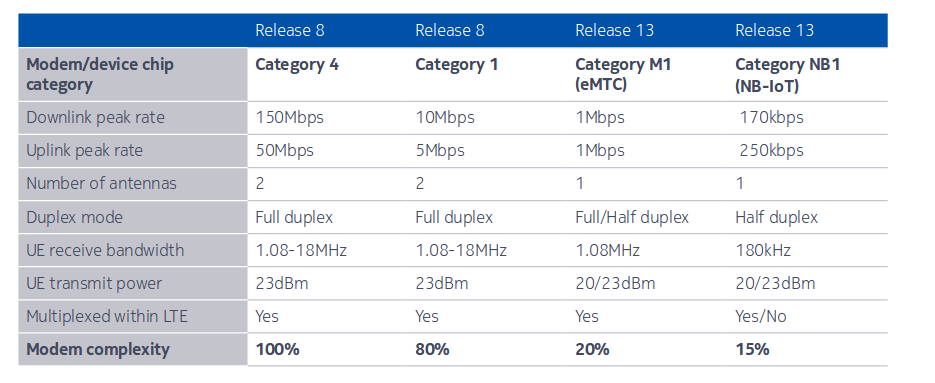
\includegraphics[width=\linewidth]{Images/Kategoriat.png}
    \caption{Taulukko päätelaitekategorioista \cite{nokiawhitepaper}.}
    \label{fig:kategoria}
\end{figure}

 \textit{Release 12}:ssa \cite{release12} M2M-päätelaitteille esiteltiin \textit{Category 0}, jonka on tarkoitus on vähentää päätelaitteiden kompleksisuutta ja energiankulutusta verrattuna \textit{Category 1}:een. \textit{Cat-0} laitekategorian lataus- ja lähetysnopeudet on laskettu 1 Mbps:iin, minkä lisäksi kategorian laitteet voivat viestiä vain yhdellä vastaanottoketjulla \cite{gsmawhitepaper}. Lisäksi vuorosuuntainen liikenne on laitteille sallittu taajuusjakoista kaksisuuntaisuutta käytettäessä. Tämän myötä aika-avaruudessa lomitetussa kaksisuuntaisessa liikenteessä ei enää tarvita erillistä suodatinta.

 \textit{Cat-0}:n päätelaitteiden vastaanottokaistan leveys on kavennettu sekä lataus- että lähetyskaistalla 1,4 MHz:iin. Muutos mahdollistaa tehokkaamman AD-muunnoksen ja puskurin pienentämisen, minkä seurauksena laitteet pystyvät toimimaan hitaammalla prosessorilla ja muistilla \cite{nokiawhitepaper}. Kaventuneesta kaistanleveydestä huolimatta laitteet voivat toimia kaikilla LTE-järjestelmän käyttämillä kaistoilla aina 20 MHz:iin asti. Virrankulutuksen vähentämiseksi \textit{Release 12}:ssa päätelaitteiden maksimilähetystehoa pudotettiin myös 20dBm:a.
 %"The active timer determines how long the device remains reachable (by checking for paging according to the regular DRX cycle) for mobile terminated transaction upon transition from connected to idle mode. The device starts the active timer when it moves from connected to idle mode. When the active timer expires, the device moves to power saving mode. In power saving mode, the device cannot be reached as it does not check for paging, but is still registered with the network. The device remains in PSM until a mobile originated transaction (e.g. periodic TAU, uplink data transmission) requires it to initiate any procedure towards the network." 

Kuten aiemmin kappaleessa todettiin, \textit{Cat-0}:n laitteet toimivat 1,4 MHz:n kantoaallolla, joka vastaa kuutta fyysistä resurssilohkoa. Kategorian päätelaite, kuten mikä tahansa muu laite, kuuntelee aina kuutta keskimmäistä resurssilohkoa, joilta laite saa kontrolli-informaation \cite{nokiawhitepaper}. Kun laitteen on vuoro liikennöidä verkossa, sille osoitetaan yhdestä kuuteen peräkkäistä resurssilohkoa käytettävältä spektriltä. Laitteelle tarkoitettu kontrolli-informaatio ja data lomitetaan taajuustasossa, ottamatta huomioon varhaisempien LTE-standardien kontrolli-informaatiota. Näin mahdollistetaan päätelaitteiden aikataulutus myös varhaisemmissa LTE-järjestelmissä.

\textit{Release 12}:ssa esiteltiin myös päätelaitteiden virransäästötila \cite{nokiawhitepaper}. Virransäästötilaa tukeva laite pyytää verkolta ajastimen verkkoon liittymisen tai paikannus (TAU, tracking area update) proseduurin aikana. \textit{Release 13}:ssa \cite{release13} julkaistiin \textit{Category M1}, jolla päätelaitteiden kompleksisuutta pyrittiin vähentämään vielä enemmän \cite{gsmawhitepaper}. Kategoria on tarkoitettu samantyyppisille sovelluksille kuin \textit{Cat-0}, ja tekniikka kulkee nimellä enhanced MTC (eMTC). Lisäksi samalla julkaistiin \textit{Category NB1} NB-IoT-verkkoteknologiaa hyödyntäville laitteille. 

%\cite{ratasuk2014ltem}

\subsection{NB-IoT}

3GPP:n \textit{Release 13}:ssa esitelty kapeakaistainen esineiden internet eli NB-IoT (Narrowband IoT) on LTE-järjestelmän valmiiden toiminnallisuuksien päälle rakennettu IoT-laitteiden verkkoteknologia. Sen tavoitteena on mahdollistaa erittäin alhaisen kompleksisuuden IoT-laitteille tuki mobiiliverkossa, 20dB parempi sisätilojen kattavuus GPRS:een verrattuna, tuki yli 52 tuhannelle samaan aikaan kytketylle laitteelle, sekä yli kymmenen vuoden akunkesto 5 Wh akuille. Lisäksi NB-IoT-järjestelmän ei tulisi haitata samalla taajuskaistalla toimivia, olemassa olevia mobiiliverkkojärjestelmiä. \cite{ratasuk2016overview}

NB-IoT tukee kolmea toimintatilaa. Se voi toimia itsenäisesti (stand-alone) hyödyntäen yhtä tai useampia GSM-kantoaaltoa, käyttäen LTE-järjestelmän kaistansisäisiä (in-band) resurssilohkoja tai LTE-järjestelmän kantoaallon suojakaistan (guard-band) sisäisiä, käyttämättömiä resurssilohkoja. Resurssilohkojen jakaminen LTE- ja NB-IoT-järjestelmien välillä mahdollistaa tehokkaamman taajuusspektrin käytön, minkä lisäksi molempien järjestelmien tuki voidaan saavuttaa samalla tukiaseman laitteistototeutuksella. GSM-kantoaaltoja käytettäessä NB-IoT pystyy hyödyntämään jo hyvin laajan kattavuuden maailmanlaajuisesti saanutta GSM-infrastruktuuria. \cite{ratasuk2016nb, ratasuk2016overview}

NB-IoT:n latauskaista on jaettu 15 kHz:n alikantoaaltoihin ja modulaatiomenetelmänä käytetään OFDMA:ta, mikä eroaa \textit{Release 8}:ssa määritellystä 20 Mhz:n kantoaallosta ja QPSK, 16QAM ja 64QAM -modulaatiomenetelmistä. \cite{ratasuk2016nb, harmaala, release8} NB-IoT:n lähetyskaista tukee 3,75 kHz:n ja 15 kHz:n alikantoaaltoja yksisuuntaisissa lähetyksissä (single-tone transmission). Kaksisuuntaisissa lähetyksissä (multi-tone transmission) tuki on 15 kHz:n alikantoaalloille ja SC-FDMA-modulaatiomenetelmälle. \cite{ratasuk2016nb}

Merkittävä muutos NB-IoT:ssa on neljän fyysisen kanavan karsiminen. NB-IoT:ssa käytössä ovat kanavat NPDCCH, NPDSCH, NPBCH, NPSS, NSSS, NPUSCH ja NPRACH, minkä johdosta \textit{Release 8}:aan verrattuna karsittujen kanavien PMCH, PCFICH, PDCCH ja PHICH sisältämä informaatio kuljetetaan jäljellä olevia kanavia pitkin \cite{ETSIts36211, harmaala}. Tämä mahdollistaa sen, että päätelaitteita voidaan yksinkertaistaa, ja vähentää niiden virrankulutusta. Tämän lisäksi verkon resurssienkäyttö tehostuu \cite{ratasuk2016nb, harmaala}.

%NB-IoT:n pääinformaatiolähetykset (MIB, Master Infromartion Broadcast) välitetään latauslinkin ensimmäisessä fyysisessä kanavassa. Pääinformaatiolähetyksessä kuljetetaan tieto niistä parametereista, joita päätelaite tarvitsee tarvitsee muodostaakseen yhteyden tukiasemaan \cite{harmaala}. Pääinformaatiolähetys on kooltaan 50 bittiä

\clearpage
\section{LTE-standardin kehityksen tulevaisuuden näkymät}

\textit{Release 13} jälkeen 3GPP:n standardoinnin pääpaino siirtyi LTE:n kehityksestä 5G:n standardointiin \cite{ericssonRelease14}. LTE-järjestelmien kehitys jatkuu taaksepäin yhteensopivien parannusten kehittämisellä olemassa olevalle radiospektrille, kun taas 5G:n kehitys keskittyy isommalle varaamatomalle radiospektrille ja uuden . Kehitystyötä tehdään tiiviissä yhteistyössä, jotta LTE-järjestelmätkin pystyvät saavutaamaan tiukkoja 5G:n edellytyksiä. 3GPP on määritellyt omiin 5G-järjestelmän edellytyksiinsä parannetun mobiililaajakaistan (eMBB), mittavan koneiden välinen kommunikaation (mMTC) ja erittäin luotettavan vähälatenssinen kommunikaation (URLLC) \cite{hoymann2016lte}.

%According to its usage, URLLC and mMTC are latency sensitive and need high reliable communication where as eMBB demands higher data rates and capacities. From these three scenarios, eMBB remains the most critical as the ongoing growth of users demanding the eMBB services proves to be strong and profitable. Requirement of the eMBB scenario is to support a much wider range of code rates, code lengths and modulation orders than the 4G Long Term Evolution (LTE). In the current assumption, eMBB code lengths range from 100 to 8000 bits (optionally 12,000-64000 bits) and code rate ranges from 1/5 to 8/9.

eMBB:n toteutuminen vaatii 5G-järjestelmältä kapasiteettia tukea kasvavaa viestiliikenteen määrää, samalla tarjoten käyttäjille kaikkialla vähintään 10 Mbps nopeuden ja 20 Gbps:n huippudatansiirtonopeuden. Tiheään rakennetut verkon tukiasemat, laajemman radiospektrin käyttö ja spektrinkäytön tehokkuuden parantaminen on välttämätön edellytys eMBB:n toteutumiselle \cite{hoymann2016lte}. Esimerkiksi tukiasemien sijoittaminen mm. lyhtypylväisiin ja lisensoimattoman radiospektrin ottaminen käyttöön ovat jo käytössä olevia menetelmiä yhteyden parantamiseksi.

mMTC:lla tarkoitetaan tukea vähäisen liikenteen ja pitkän akunkeston laitteille, kuten sensoreille ja vastaaville laitteille \cite{hoymann2016lte}. mMTC asettaa haasteita verkon kattavuudelle ja signaalinkäsittelylle. Tässä kandidaatintyössä kappaleessa 3 esitetyt LTE-M- ja NB-IoT-teknologiat osaltaan vastasivat jo mMTC:n asettamiin haasteisiin, mutta kehityksen on tarkoitus jatkua tulevissa 3GPP:n julkaisuissa.

URLLC:lla tarkoitetaan kommunikaatioyhteyden latenssin ja luotettavuuden parantamista. Luotettava ja matalan latenssin kommunikaatio mahdollistaa muun muassa uusien terveys-, turvallisuus- ja hallintapalveluiden toteuttamisen esineiden internetin avulla \cite{hoymann2016lte}. Esimerkiksi \textit{Release 14}:ssa esitelty älykäs liikennejärjestelmä (ITS) vaatii toimiakseen luotettavan LTE-kommunikaation \cite{ericssonITS}.

\subsection{Release 14}

LTE-järjestelmien kehitys jatkui \textit{Release 14}:ssä \cite{release14} latenssien vähentämisellä, sekä lisensoimattoman spektriin, M2M-kommunikaatioon ja MIMO-tekniikkaan liittyvillä parannuksilla \cite{ericssonRelease14}. Latenssia on piennennetty mahdollistamalla lähetyskaistalla lähettäminen osalle laitteista ilman aikataulutuspyyntöjä. \cite{hoymann2016lte} Konventionaalisesti päätelaitteen täytyy pyytää tukiasemalta lupa datan lähettämiselle, jolloin lähetyksessä vältytään aikataulutuspyynnön ja lähetyskaistan myöntämisen aiheuttamalta viiveeltä ja round-trip-viiveajalta (Kuva \ref{fig:URLLC}).

~\begin{figure}[h!]
    \centering
    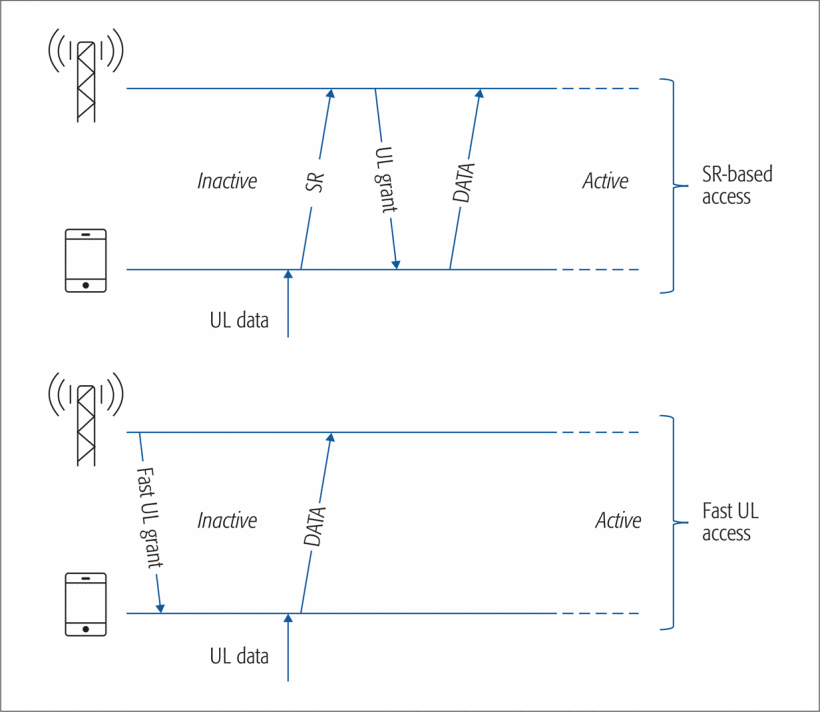
\includegraphics[scale=0.4]{Images/URLLC.png}
    \caption{Aikataulutuspohjainen yhteys (ylhäällä) ja nopean lähetyskaistan yhteys (alhaalla) \cite{hoymann2016lte}.}
    \label{fig:URLLC}
\end{figure}

NB-IoT koki myös parannuksia \textit{Release 14} ja \textit{Release 15}:ssa \cite{release15}. Päätelaitteen paikannusta parannettiin esittelemällä kolme paikannustapaa \textit{Release 13}:ssa esitellyn soluidentiteettipaikannuksen sijaan (CID) \cite{ratasuk2017enhancements}. Parannetussa E-CID --paikannuksessa hyödynnetään lähetys- ja vastaanottoaikojen aikaeroa, sekä referenssisignaalin vastaanottotehoa ja -laatua \cite{hoglund2017overview}. OTDOA-paikannuksessa päätelaite mittaa latauslinkillä usealta lähettävältä tukiasemalta uuden paikannusreferenssisignaalin (NPRS) ToA-aikoja. Mittauksista muodostetaan geograafisia hyberbolia, joiden risteyskohdassa päätelaitteen voidaan päätellä sijaitsevan \cite{hoglund2017overview}.

Uusi päätelaitekategoria \textit{Cat-NB2} esiteltiin tukemaan moninaisempia radioliikenneskenaarioita \cite{hoglund2017overview}. Uuden kategorian laitteet on tarkoitettu suotuisemmissa radio-olosuhteissa oleville laitteille. Kategorian laitteet pääsevät nopeampiin huippudatansiirtonopeuksiin 2536 bittiin kasvatetun TBS:n ja toisen HARQ-prosessiin tuen puolesta. Lisäksi \textit{Release 14}:ssa paranneltiin tukiasemien monilähetystä, jonka avulla usean älykkään laitteen samanaikainen ohjelmistopäivitys on mahdollista, sekä usealle laitteelle kommunikoinnin latenssia saatiin pienennettyä.

\subsection{Release 15}

\textit{Release 15}:ssa konetyyppisten laitteiden kommunikaatiota parannettiin pienentämällä latenssia ja virrankulutusta, sekä lisättiin tuki aikajakoiselle kaksisuuntaisuudelle \cite{ratasuk2017enhancements}. 

latency reduction, power consumption reduction

TDD support, NPRACH enchaned

Fyysinen layer päätetty, 5G new radio. Katso tavoitteita.

\subsection{LTE lisensoimattomalla spektrillä}

LTE-verkkojen nopeasti kasvava liikenteen määrä on houkuttelee operoimaan LTE-järjestelmiä 5 GHz:n lisensoimattomalla radiospektrillä. Lisensoimattomalla spektrillä verkon kapasiteettia on halvempaa kasvattaa kuin lisensoidulla kaistalla. Tällä hetkellä kriittisin ongelma 5 GHz:n kaistan käyttämiselle on se, että samalla kaistalla toimii Wi-Fi -teknologia~\cite{ismaiel2017survey}. Joidenkin tutkimusten mukaan samalla kaistalla toimivat teknologiat saattavat häiritä toisiaan ja heikentää molempien verkkojen toimintaa~\cite{naik2018coexistence, ismaiel2017survey}.

Ensimmäinen lisensoimattomalla spektrillä toimiva LTE-teknologia, LTE unlicensed (LTE-U), perustui LTE:n \textit{Release 12}:een. LTE-U standardista kuitenkin puuttuu niin sanottu \textit{kuuntele ennen lähettämistä} -tekniikka (LBT), joka on vaatimus Euroopassa ja Japanissa radiotekniikoille, jotka käyttävät lisensoimatonta radiospektriä. LTE-U:iin perustuva LTE-Licensed Assisted Access (LTE-LAA) standardoitiin 3GPP:n toimesta \textit{Release 13}:ssa, ja standardiin kuului myös LBT-tekniikka. \textit{Release 13}:ssa esiteltiin myös LTE Wi-Fi Aggregation (LWA), joka mahdollistaa Wi-Fi-tukiasemien hyödyntämisen LTE-tekniikalle. LWA toimii siten, että osa LTE:n liikenteestä siirretään Wi-Fi:n kautta käyttäen CSMA-protokollaa.~\cite{ismaiel2017survey}
~\begin{figure}[h!]
    \centering
    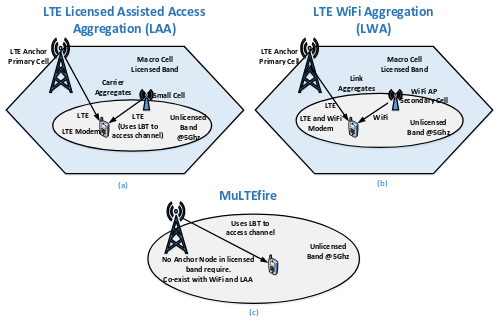
\includegraphics[scale=0.5]{Images/unlicensed.png}
    \caption{LTE lisensoimattomalla spektrillä~\cite{ismaiel2017survey}.}
    \label{fig:unlicensed}
\end{figure}

MulteFire on MulteFire Alliancen kehittämä LTE-pohjainen tekniikka, joka toimii täysin lisensoimattomalla radiospektrillä. Se perustuu 3GPP:n \textit{Release 13}:ssa ja \textit{Release 14}:ssa esiteltyihin LAA- ja eLAA-tekniikoihin \cite{chambers2016multefire}, mutta eroaa näistä siten, että se ei tarvitse ankkuritukiasemaa lisensoidulta radiospektriltä \cite{ismaiel2017survey, multefire2015lte}. MulteFire hyödyntää LBT-tekniikkaa, joten se voi toimia samassa ympäristössä esimerkiksi Wi-Fi- ja LAA-järjestelmien kanssa. Koska MulteFire perustuu LTE-järjestelmään, se toimii 20 MHz:n alikaistoilla, joista se osaa eLAA:n tapaan dynaamisesti valita vähiten käytetyimmät kanavat \cite{chambers2016multefire}. Dynaaminen alikaistanvalinta vähentää muihin radiospektriä käyttäviin järjestelmiin aiheutuvia häiriöitä.
~\begin{figure}[h!]
    \begin{minipage}{0.5\textwidth}
        \centering
        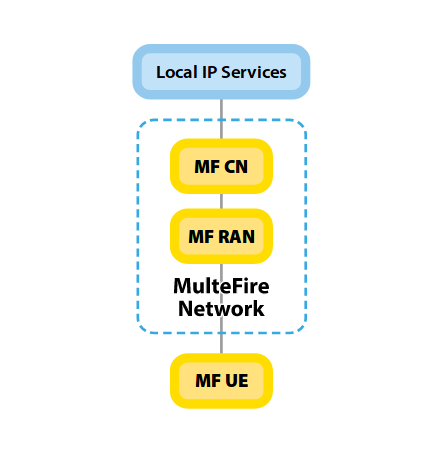
\includegraphics[width=0.5\linewidth]{Images/MF1.png}
        \caption{Itsenäinen toimintatila~\cite{chambers2016multefire}.}
        \label{fig:MF1}
    \end{minipage}
    \begin{minipage}{0.5\textwidth}
        \centering
        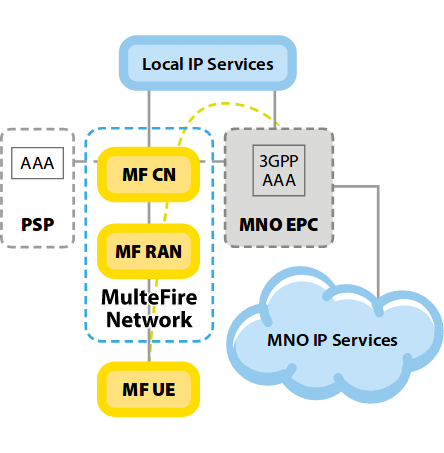
\includegraphics[width=0.5\linewidth]{Images/MF2.png}
        \caption{Itsenäinen verkko verkkovierailutuella ulkoisille mobiiliverkoille~\cite{chambers2016multefire}.}
        \label{fig:MF2}
    \end{minipage}
\end{figure}

MulteFire tukee kolmea toimintatilaa. Itsenäisessä toimintatilassa (Kuva \ref{fig:MF1}) MulteFire tukiasemat muodostavat yksityisen ja omavaraisen verkon. Verkon laitteet eivät tarvitse omaa SIM-korttia, mutta verkosta löytyy tuki virtuaalisille tai yksityisille SIM-korteille \cite{chambers2016multefire}. Kuvan \ref{fig:MF2} verkko toimii muuten samoin kuin itsenäinen MulteFire-verkko, mutta verkko toimii myös neutraalina verkkovierailupalveluntarjoajana ulkoisten operaattorien verkojen käyttäjille. Kolmannessa toimintatilassa MulteFiren verkko toimii osana operaattorin mobiiliverkkoa. Olemassa olevia SIM-kortteja käytetään verkkoon yhdistäessä. MulteFiren voi tukea kaikkia mahdollisia toimintatilojen kombinaatioita samanaikaisesti. Tämä on hyödyllistä esimerkiksi erottaessa vierailijaverkot henkilökuntaverkoista.
~\begin{figure}[h!]
    \centering
    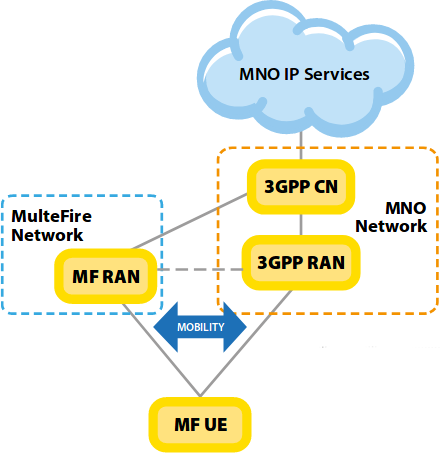
\includegraphics[scale=0.25]{Images/MF3.png}
    \caption{Ulkoisiin mobiiliverkkoihin tiukasti integroitu verkko~\cite{chambers2016multefire}.}
    \label{fig:MF3}
\end{figure}

MulteFiren julkaisuversiossa 1.1 on valmistumassa kesäkuussa 2018 \cite{multefire11}. Julkaisussa MulteFirea on optimoitu IoT-laitteiden käyttöön, sekä LTE-järjestelmistä tutut eMTC- ja NB-IoT-tekniikat on lisätty MulteFiren standardiin. NB-IoT-laitteet voivat \textit{MulteFire 1.1}:ssä toimia alle 1 GHz:n, 1,9 GHz:n ja 2.4 GHz:n radiospektrillä. eMTC-laitteet voivat toimia näiden lisäksi vielä 3.5 GHz:n radiospektrillä. Päivityksen myötä \textit{MulteFire 1.1} vastaa pitkälti LTE-standardin \textit{Release 14}:ä. MulteFiren kehitys jatkuu rinnakkaisena LTE:n kehityksren kanssa.

\clearpage
\section{Yhteenveto}
%\section{Summary}

\clearpage
%% Lähdeluettelo
%%
%% \phantomsection varmistaa, että hyperref-paketti latoo hypertekstilinkit
%% oikein.
%%
%% The \phantomsection command is nessesary for hyperref to jump to the 
%% correct page, in other words it puts a hyper marker on the page.

\phantomsection{}
\addcontentsline{toc}{section}{Viitteet}
%\addcontentsline{toc}{section}{References}

\printbibliography{}

%% Liitteet 
%\appendix 
\clearpage
%% Lisää tekstin "Liitteet" sisällysluetteloon
%%
%% Adds the word "Appendices" to the table of contents
%\addtocontents{toc}{\protect\contentsline{section}{Liiteet}{}{appendix}}
%\addtocontents{toc}{\protect\contentsline{section}{Appendices}{}{appendix}}

%\section{Esimerkki liitteestä\label{LiiteA}}
%% Liitteiden kaavat, taulukot ja kuvat numeroidaan omana kokonaisuutenaan
%%
%% Equations, tables and figures have their own numbering in Appendices
%\renewcommand{\theequation}{A\arabic{equation}}
%\setcounter{equation}{0}  
%\renewcommand{\thefigure}{A\arabic{figure}}
%\setcounter{figure}{0}
%\renewcommand{\thetable}{A\arabic{table}}
%\setcounter{table}{0}

%Liitteet eivät ole opinnäytteen kannalta välttämättömiä ja opinnäytteen tekijän on kirjoittamaan ryhtyessään hyvä ajatella pärjäävänsä ilman liitteitä.Kokemattomat kirjoittajat, jotka ovat huolissaantekstiosan pituudesta, paisuttavat turhan helposti liitteitä pitääkseen tekstiosan pituuden annetuissa rajoissa.Tällä tavalla ei synny hyvää opinnäytettä.   

%Liite on itsenäinen kokonaisuus, vaikka se täydentääkin tekstiosaa.Liite ei siten ole pelkkä listaus, kuva tai taulukko, vaan liitteessä selitetään aina sisällön laatu ja tarkoitus. 

%Liitteeseen voi laittaa esimerkiksi listauksia. Alla on listausesimerkki tämän liitteen luomisesta. 

%% Verbatim-ympäristö ei muotoile tai tavuta tekstiä. Fontti on monospace.
%% Verbatim-ympäristön sisällä annettuja komentoja ei LaTeX käsittele. 
%% Vasta \end{verbatim}-komennon jälkeen jatketaan käsittelyä.

\end{document}
